\documentclass[a4paper,12pt]{report}
\usepackage[T2A]{fontenc}
\usepackage[utf8]{inputenc}
\usepackage[english,russian]{babel}
\usepackage{graphicx}
\usepackage{wrapfig}
\usepackage{mathtext} 				% русские буквы в фомулах
\usepackage{amsmath,amsfonts,amssymb,amsthm,mathtools} % AMS
\usepackage{icomma} % "Умная" запятая: $0,2$ --- число, $0, 2$ --- перечисление
\usepackage{capt-of}
\usepackage{appendix}
\usepackage{multirow}
\usepackage{hyperref}
\usepackage[left=3cm,right=3cm, bottom=3cm]{geometry}
\usepackage{multicol} % Несколько колонок
\usepackage{gensymb}
\title{Отчёт по лабораторной работе №3.7.1 

Скин-эффект в полом цилиндре.}
\author{Плюскова Н.А. Б04-004 }


\begin{document}

\maketitle

\section*{\huge{Описание работы}}

\noindent\textbf{Цель работы:} исследование проникновения переменного магнитного поля в медный полый цилиндр.

\noindent\textbf{В работе используются:} генератор звуковой частоты, соленоид, намотанный на полый цилиндрический каркас из диэлектрика, медный экран в виде трубки, измерительная катушка, амперметр, вольтметр, осциллограф.

\vspace{\baselineskip}
\noindent\textbf{Теоретические сведения}

Возьмем цилиндр достаточно длинный для того, чтобы в нем можно было пренебречь краевыми эффектами. В этом приближении поле $H$ всюду направлено по оси системы (ось $z$), а вихревое электрическое поле $E$ будет всюду перпендикулярно радиусу, т.е. линии поля образуют соосные окружности (рис.1). Все величины будем считать колеблющимися по гармоническому закону с некоторой частотой $w$, задаваемой частотой колебаний тока в соленоиде. Тогда для ненулевых компонент поля можно записать:
\begin{gather*}
  H_{z} = H(r)e^{iwt}, \
  E_{\varphi} = E(r)e^{iwt},
\end{gather*}
где $H(r)$ и $E(r)$ - комплексные амплитуды колебаний соответствующих полей, зависящие только от расстояния $r$ до оси системы. Заметим, что на границе цилиндра должны быть непрерывны касательные к поверхности компоненты как $E$, так и $B$, поэтому функции $E(r)$ $H(r)$ непрерывны во всей исследуемой области.

\begin{center}
	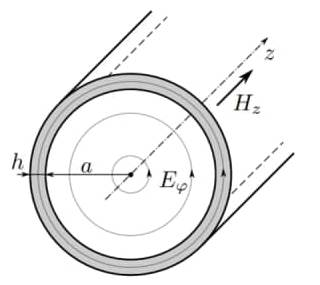
\includegraphics[width=0.3\textwidth]{рис1.jpg}\\
	\caption{Рис.1: Электрическое и магнитное поле в тонкостенном цилиндре}
\end{center}

Пусть длинный полый цилиндр имеет радиус $a$ и толщину стенки $h \ll a$. Последнее условие позволяет для описания поля внутри стенки ограничиться одномерным приближением. При этом для полного решения задачи необходимо вычислить и распределение поля внутри цилиндра.

Поскольку внутри цилиндра ток отсутствует, магнитное поле там является однородным (аналогично полю внутри пустого соленоида): \(H_{z}(r,t) = H_{1} e^{iwt}\), где \(H_{1}=const\) - амплитуда поля на внутренней поверхности цилиндра. Для нахождения вихревого электрического поля воспользуемся законом электромагнитной индукции: \(rot E = -\frac{\partial B}{\partial t}\)
\begin{gather*}
    2\pi\cdot rE_{\varphi} = -\mu_{0}\pi r^2\frac{dH_{z}}{dt} \rightarrow
    E(r) = -\frac{1}{2}\mu_{0}r\cdot iwH_{1}
\end{gather*}
Отсюда получаем связь амплитуд колебаний электрического и магнитного полей на внутренней (\(r=a\)) границе цилиндра:
\begin{equation}
    E_{1} = -\frac{1}{2}iwa\mu_{0}H_{1}.
\end{equation}
Соотношение (1) используем далее как дополнительное граничное условие для задачи о распределении поля внутри стенки.

Поле внутри тонкой стенки цилиндра ("экрана") описывается уравнением скин-эффекта: \( \frac{\partial^2 E_{y}}{\partial x^2}=\sigma\mu\mu_{0}\frac{\partial E_{y}}{\partial t}\) (уравнением диффузии поля) в плоской геометрии (рис.2). Поместим начало отсчета на внешнюю поверхность цилиндра и направим оси $x$ к оси системы, и запишем дифференциальное уравнение для комплексной амплитуды магнитного поля:
\begin{equation}
    \frac{\partial^2 H}{\partial x^2} = iw\sigma\mu_{0}H
\end{equation}
(для медного цилиндра можно положить \(\mu\approx 1\))
\begin{center}
	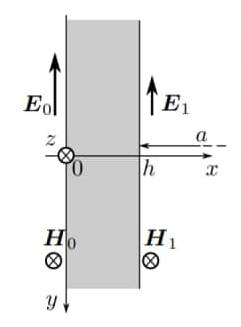
\includegraphics[width=0.3\textwidth]{рис2.jpg}\\
	\caption{Рис.2: Поле в стенке цилиндра}
\end{center}
Граничные условия для (2) зададим в виде
\begin{gather}
    H(0)=H_{0},\
    H(h)=H_{1}.
\end{gather}
Здесь $H_{0}$ - амплитуда колебаний магнитного поля на внешней границе цилиндра. Ее значение определяется только током в обмотке соленоида, и совпадает с полем внутри соленоида в отсутствие цилиндра. Величина $H_{1}$ также поддается непосредственному измерению - это амплитуда колебаний однородного поля внутри цилиндра Поля $H_{0}$ и $H_{1}$ не являются независимыми - они связаны через решение уравнений поля вне проводника, т.е. внутри "экрана". Эта связь выражена соотношением (1).

Решение (2) ищем в виде
\begin{equation}
    H(x) = Ae^{\alpha x} + Be^{-\alpha x},
\end{equation}
где A,B - определяемые из граничных условий константы,
\begin{equation}
    \alpha = \sqrt{iw\sigma\mu_{0}} = \frac{1+i}{\delta}=\frac{\sqrt{2}}{\delta}e^{i\frac{\pi}{4}}
\end{equation}
- один из корней уравнения \(\alpha^2 = iw\sigma\mu\mu_{0}\), $\delta$ - глубина скин-слоя (\(\delta=\sqrt{\frac{2}{w\sigma\mu\mu_{0}}}=\sqrt{\frac{2D}{w}}\)).

Первое условие (3) дает \(A+B=H_{0}\), что позволяет исключить $A$ из (4):
\begin{equation*}
    H(x) = H_{0}e^{-\alpha x} + 2B sh\alpha x.
\end{equation*}
Выразим электрическое поле из закона Ампера (\(rot H = \sigma E\)). В одномерном случае
\begin{equation*}
    E(x) = \frac{1}{\sigma}\frac{dH}{dx} = \frac{\alpha}{\sigma}(-H_{0}e^{-\alpha x} + 2B ch\alpha x). 
\end{equation*}
Далее положим \(x=h\), воспользуемся условием (1), и, исключив константу $B$, получим после преобразований связь между $H_{0}$ и $H_{1}$:
\begin{equation}
    H_{1} = \frac{H_{0}}{ch\alpha h + \frac{1}{2} \alpha a sh(\alpha h)}.
\end{equation}

Рассмотрим предельный случай (6).

1. При \textit{малых частотах} толщина скин-слоя превосходит толщину цилиндра \(\delta \gg h\). Тогда \(|\alpha h| \ll 1\), поэтому \(ch\alpha h \approx 1, sh \alpha h \approx \alpha h\) и 
\begin{equation}
    H_{1} \approx \frac{H_{0}}{1 + i\frac{ah}{\delta^2} }.
\end{equation}
Заметим, что величина \(ah/\delta^2\) в общем случае не мала, поскольку при \(h\ll a\) возможна ситуация \(h\ll \delta\ll a\). Отношение модулей амплитуд здесь будет равно
\begin{equation}
   \frac{H_{1}}{H_{0}} = \frac{1}{\sqrt{1 + (\frac{ah}{\delta^2})^2 }} = \frac{1}{\sqrt{1+\frac{1}{4}(\alpha h\sigma\mu_{0} w)^2}}.
\end{equation}
При этом колебания $H_{1}$ отстают по фазе от $H_{0}$ на угол $\phi$, определяемый равенством \(tg\phi = \frac{ah}{\sigma^2}\)

2. При достаточно \textit{больших частотах} толщина скин-слоя станет меньше толщины стенки: \(\delta\ll h\). Тогда \(|\alpha h| \gg 1\) и \(|\alpha a| \gg 1\), а также \(sh(\alpha h)\approx ch(\alpha h)\approx \frac{1}{2}e^{\alpha h}\). Выражение (6) с учетом (5) переходит в 
\begin{equation}
   \frac{H_{1}}{H_{0}} = \frac{4}{\alpha a}e^{-\alpha h} = \frac{2\sqrt{2}\delta}{a}e^{-\frac{h}{\delta}}e^{-i(\frac{\pi}{4}+\frac{h}{\delta})}.
\end{equation}
Как видно из формулы (9), в этом пределе поле внутри цилиндра по модулу в \(\frac{2\sqrt{2}\delta}{a} e^{-\frac{h}{\delta}}\) раз меньше, чем снаружи, и, кроме того, запаздывает по фазе на
\begin{equation}
   \phi = \frac{\pi}{4}+\frac{h}{\delta}=\frac{\pi}{4}+h\sqrt{\frac{w\sigma\mu_{0}}{2}}.
\end{equation}

На рис.3 схематично изображено распределение магнитного поля от координаты в двух рассмотренных предельных случаях.

\begin{center}
	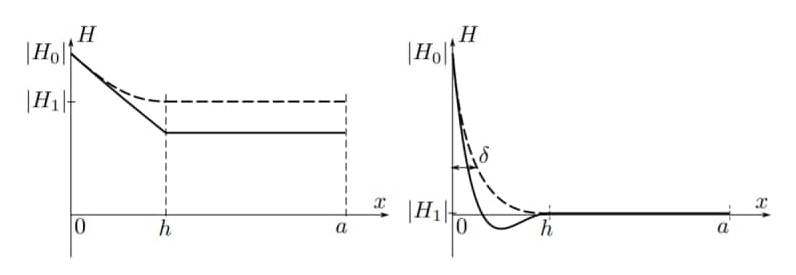
\includegraphics[width= 1\textwidth]{рис3.jpg}\\
	\caption{Рис.3: Распределение амплитуды колебаний магнитного поля (пунктир) и его мгновенного значения при некотором t (сплошная) в зависимости от расстояния до внешней стенки цилиндра. Слева случай низких частот (\(\delta\gg h\)), справа - скин-эффект при высоких частотах (\(\delta\ll h\))}
\end{center}

\vspace{\baselineskip}
\noindent\textbf{Экспериментальная установка}

Схема экспериментальной установки для исследования проникновения переменного магнитного поля в медный полый цилиндр изображена на рис.4. Переменное магнитное поле создается с помощью соленоида, намотанного на полый цилиндрический каркас 1 из поливинилхлорида, который подключается к генератору звуковой частоты. Внутри соленоида расположен медный цилиндрический экран 2. Для измерения магнитного поля внутри экрана используется катушка 3. Действующее значение переменного тока в цепи соленоида измеряется амперметром А, а действующее значение напряжения на измерительной катушке измеряет вольтметр V. Для измерения сдвига фаз между током в цепи соленоида и напряжением на измерительной катушке используется двухканальный осциллограф. На вход одного канала подается напряжение с резистора R, которое пропорционально току, а на вход второго канала - напряжение с измерительной катушки.
\begin{center}
	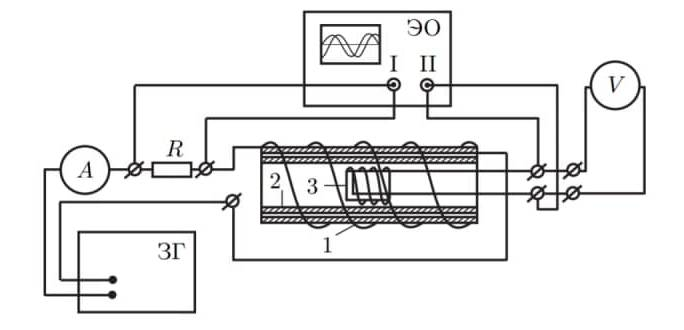
\includegraphics[width=0.8\textwidth]{рис4.jpg}\\
	\caption{Рис.4: Экспериментальная установка для изучения скин-эффекта}
\end{center}
\textbf{Измерение отношения амплитуд магнитного поля внутри и вне экрана.} С помощью вольтметра V измеряется действующее значение ЭДС индукции, которая возникает в измерительной катушке, находящейся в переменном магнитном поле \(H_{1}e^{iwt}\). Комплексная амплитуда ЭДС индукции в измерительной катушке равна 
\begin{equation*}
   U=-SN\frac{dB_{1}(t)}{dt} = -wi\mu_{0}SNH_{1}e^{iwt},
\end{equation*}
где SN - произведение площади витка на число витков измерительной катушки. Показание вольтметра, измеряющего это напряжение:
\begin{equation*}
   U=\frac{SNw}{\sqrt{2}}\mu_{0}|H_{1}|.
\end{equation*}
Видно, что модуль амплитуды магнитного поля внутри экрана $|H_{1}|$ пропорционален $U$ и обратно пропорционален частоте сигнала \(\nu=\frac{w}{2\pi}\):
\begin{equation*}
   |H_{1}|\propto \frac{U}{\nu}.
\end{equation*}
При этом  поле вне экрана $|H_{0}|$ пропорционально току $I$ в цепи соленоида, измеряемому амперметром А:
\begin{equation*}
   |H_{0}|\propto I.
\end{equation*}
Следовательно,
\begin{equation}
   \frac{|H_{1}|}{|H_{0}|}=const\cdot \frac{U}{\nu I}.
\end{equation}

Таким образом, отношение амплитуд магнитных полей снаружи и вне экрана (коэффициент ослабления) может быть измерено по отношению \(\frac{U}{\nu I}\) при разных частотах. Неизвестная константа в соотношении (11) может быть определена по измерениям при малых частотах \(\nu \rightarrow 0\), когда согласно (8) \(\frac{|H_{1}|}{|H_{0}|}\rightarrow 1\).

\textbf{Определение проводимости материала экрана.} В установке в качестве экрана используется медная труба промышленного производства. Технология изготовления труб оказывает заметное влияние на электропроводимость. Из-за наличия примесей проводимость меди нашей трубы отличается от табличного значения (в меньшую сторону). Для определения $\sigma$ нашего экрана предлагается использовать частотную зависимость (10) фазового сдвига между магнитными полями внутри и вне экрана при высоких частотах. Как видно из выражения (10), в области больших частот \(w \gg \frac{1}{h^2\sigma\mu_{0}}\) зависимость \(\phi(\sqrt{w})\) аппроксимируется прямой, проходящей через точку \(\phi(0)=\frac{\pi}{4}\). По наклону этой прямой можно вычислить проводимость материала экрана.

Заметим, что на схеме, изображенной на рис.4, на входной канал II осциллографа подается сигнал с измерительной катушки, который пропоционален не полю внутри экрана, а его производной по времени, а это означает, что появляется дополнительный сдвиг по фазе на $\pi/2$. Поэтому измеренный по экрану осциллографа сдвиг по фазе между двумя синусоидами будет на $\pi/2$ больше фазового сдвига между магнитными полями вне и внутри экрана.


\section*{\huge{Выполнение работы}}
\noindent\textbf{Параметры установки:}

$a = 21$мм - радиус цилиндра

$h = 1,3$мм - толщина стенок

По известным параметрам установки, приняв проводимость меди для оценки равной \(\sigma\sim 5\cdot10^7\) См/м, рассчитаем $\nu_{h}$ - частоту, соответствующую равенству \(h=\delta\) толщины стенок экрана скиновой длине:

\begin{equation*}
    \nu_{h} = \frac{1}{\pi\sigma\mu\mu_{0}h^2}= \frac{1}{3,14\cdot5\cdot10^7\cdot1,26\cdot10^{-6}\cdot1,3\cdot10^{-6}\text{См/м}\cdot\text{Гн/м}\cdot\text{м}^2}\approx 3,8\cdot10^3 \text{Гц}
\end{equation*}


В области низких частот 20–100 Гц (с шагом 5 Гц) снимем зависимость «амплитуды» $\varepsilon_{0c}$ (\(\varepsilon_{0c}=\frac{U}{fI}\)) магнитного поля внутри экрана от частоты (см. Таблицу 1).

\begin{table}[!ht]
    \centering
    \begin{tabular}{|p{1cm}|p{1.3cm}|p{1.3cm}|p{1.3cm}|p{1.3cm}|p{1cm}|p{1.7cm}|}
    \hline
        f, Гц & $\sigma_{f}$, Гц & I, мА & $\sigma_{I}$, мА & U, В & $\sigma_{U}$, В&$\varepsilon_{0c}$, кГн \\ \hline
        20 & 0.25 & 53.3 & 6 & 0.0119 & 0.36&0.0112 \\ \hline
        25 & 0.25 & 53.5 & 6 & 0.0145 & 0.36&0.0108 \\ \hline
        30 & 0.25 & 53.6 & 6 & 0.0179 & 0.36&0.0111 \\ \hline
        35 & 0.5 & 53.65 & 6 & 0.0207 & 0.36&0.0110 \\ \hline
        40 & 0.5 & 53.6 & 6 & 0.0234 & 0.36&0.0109 \\ \hline
        45 & 0.5 & 53.7 & 6 & 0.0263 & 0.36&0.0109 \\ \hline
        50 & 0.5 & 54.8 & 6 & 0.029 & 0.36&0.0106 \\ \hline
        55 & 0.5 & 54 & 6 & 0.0322 & 0.36&0.0108 \\ \hline
        60 & 0.5 & 54.2 & 6 & 0.0346 & 0.36&0.0106 \\ \hline
        65 & 1 & 54.1 & 6 & 0.037 & 0.36&0.0105 \\ \hline
        70 & 1 & 53.9 & 6 & 0.0398 & 0.36&0.0105 \\ \hline
        75 & 1 & 53.95 & 6 & 0.0425 & 0.36&0.0105 \\ \hline
        80 & 1 & 53.95 & 6 & 0.045 & 0.36&0.0104 \\ \hline
        85 & 1 & 53.82 & 6 & 0.0477 & 0.36&0.0104 \\ \hline
        90 & 1 & 53.86 & 6 & 0.05 & 0.36&0.0103 \\ \hline
        95 & 1 & 53.8 & 6 & 0.0529 & 0.36&0.0104 \\ \hline
        100 & 1 & 53.69 & 6 & 0.0548 & 0.36&0.0102 \\ \hline
    \end{tabular}
\begin{center}
\caption{Данные, полученные на низких частотах}
\end{center}
\end{table}
Построим график в координатах $\varepsilon_{0c}$ от $f^2$ и аппроксимируем полученную зависимость прямой.

\begin{center}
	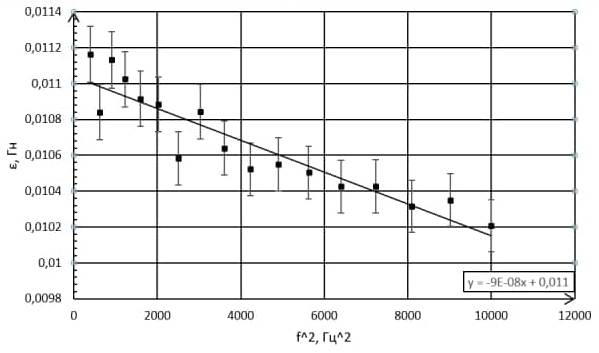
\includegraphics[width=0.9\textwidth]{малые частоты.jpg}
\end{center}

Из графика видно, что \( \varepsilon_0 = 0,0111 \pm 0,001\) Гн

Исследуем зависимость $\varepsilon_{0c}$ и фазового сдвига $\Delta \psi$ от частоты в диапазоне 100 Гц–30 кГц (см. Таблицу 2)

\begin{table}[!ht]
\begin{tabular}{|c|c|c|c|c|c|c|c|}
\hline
f, Гц & сигма f, Гц & I, мА & сигма I & U, В   & сигма U, В & $\Delta \psi$ & $\varepsilon\phi$, \% \\ \hline
100   & 1           & 53,69 & 6       & 0,0548 & 0,36       & 0,63      & 0,17           \\ \hline
500   & 5           & 52,95 & 6       & 0,1395 & 0,36       & 0,86      & 0,17           \\ \hline
1000  & 10          & 53,88 & 6       & 0,1552 & 0,36       & 0,96      & 0,17           \\ \hline
2000  & 25          & 54,43 & 6       & 0,1605 & 0,36       & 1,00      & 0,17           \\ \hline
3000  & 25          & 54,03 & 6       & 0,16   & 0,36       & 1,05      & 0,17           \\ \hline
4000  & 50          & 53,63 & 6       & 0,159  & 0,36       & 1,14      & 0,17           \\ \hline
5000  & 50          & 53,12 & 6       & 0,1573 & 0,36       & 1,04      & 0,17           \\ \hline
6000  & 50          & 52,57 & 6       & 0,1555 & 0,36       & 1,11      & 0,17           \\ \hline
7000  & 100         & 51,88 & 6       & 0,1533 & 0,36       & 1,13      & 0,17           \\ \hline
8000  & 100         & 51,13 & 6       & 0,1512 & 0,36       & 1,14      & 0,17           \\ \hline
9000  & 100         & 50,3  & 6       & 0,1486 & 0,36       & 1,25      & 0,17           \\ \hline
10000 & 100         & 49,32 & 6       & 0,146  & 0,36       & 1,09      & 0,17           \\ \hline
12000 & 125         & 47,25 & 6       & 0,1403 & 0,36       & 1,26      & 0,17           \\ \hline
14000 & 125         & 44,62 & 6       & 0,1346 & 0,36       & 1,30      & 0,17           \\ \hline
16000 & 250         & 41,6  & 6       & 0,1285 & 0,36       & 1,33      & 0,17           \\ \hline
18000 & 250         & 38,8  & 6       & 0,1237 & 0,36       & 1,38      & 0,17           \\ \hline
20000 & 250         & 36,2  & 6       & 0,125  & 0,36       & 1,48      & 0,17           \\ \hline
22000 & 250         & 32,04 & 6       & 0,119  & 0,36       & 1,52      & 0,17           \\ \hline
24000 & 250         & 27,18 & 6       & 0,113  & 0,36       & 1,52      & 0,17           \\ \hline
26000 & 250         & 22,09 & 6       & 0,107  & 0,36       & 1,50      & 0,17           \\ \hline
28000 & 250         & 16,5  & 6       & 0,1008 & 0,36       & 1,60      & 0,17           \\ \hline
30000 & 250         & 10,8  & 6       & 0,095  & 0,36       & 1,63      & 0,17           \\ \hline
\end{tabular}
\begin{center}
\caption{Данные, полученные на высоких частотах}
\end{center}
\end{table}

Изобразим на графике в координатах $\Delta \psi$ и $\sqrt{f}$ частотную зависимость фазового сдвига $\Delta \psi$. Через точку $(0, \pi / 4)$ проведем прямую, которая касается экспериментальной кривой при больших частотах. По наклону этой прямой вычислим значение проводимости материала экрана. 

\begin{center}
	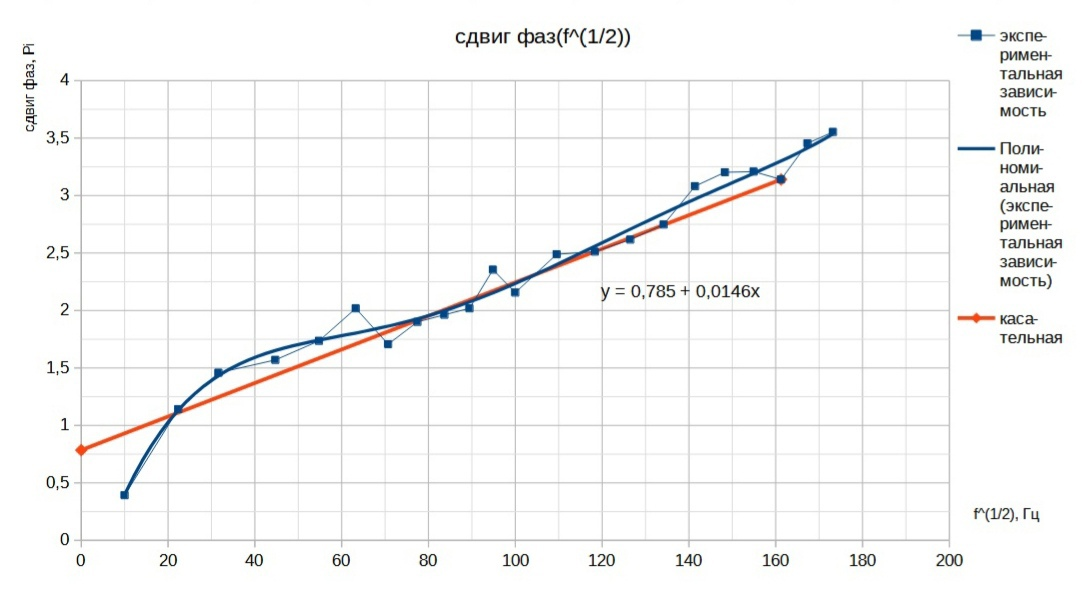
\includegraphics[width=1.0\textwidth]{большие частоты.jpg}
\end{center}

Получаем \( \sigma = (32 \pm 7) \cdot 10^6 \text{ См/м}\). Данное значение отличается от табличного в 4$\sigma_{\sigma}$ раз.

В области высоких частот изобразим зависимость $\frac{|H_{0c}|}{|H_0|}$ от $\sqrt{f}$. Используя формулу (6), рассчитаем аналогичную теоретическую зависимость и построим ее на том же графике.

\begin{center}
	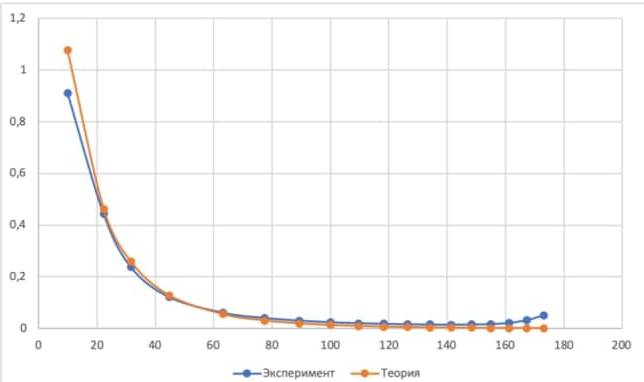
\includegraphics[width=1.0\textwidth]{третий график.jpg}
\end{center}

4) Используя найденное значение проводимости, вычислим глубину проникновения поля. При 50 Гц $\delta \approx 12 \text{ мм}$, при $10^5$ Гц $\delta \approx 281 \text{ мкм}$.

\noindent\textbf{Вывод}

В данной лабораторной работе был исследовано проникновение переменного магнитного поля в медный полый цилиндр. На основании полученных данных посчитана проводимость меди, из которой изготовлен полый цилиндр. Полученный результат в пределах 4\(\sigma\) сходится с теоретическими значениями. Вероятной причиной расхождения могут быть примеси в меди, из которой изготовлен исследуемый образец.
\end{document}
